\documentclass[11pt]{article}
\usepackage[a4paper,margin=2.5cm]{geometry}
\usepackage{amsmath,amssymb,amsthm,graphicx,booktabs,xcolor}
\usepackage[colorlinks=true,linkcolor=blue!60!black,citecolor=blue!60!black,urlcolor=blue!60!black]{hyperref}
\usepackage{xurl}
\hypersetup{pdftitle={Crossover from Discrete to Continuous Quantum Geometry},pdfauthor={Ruqing Chen}}
\setlength{\emergencystretch}{3em}
\graphicspath{{../figures/}{figures/}{./}}

\newtheorem{theorem}{Theorem}
\newtheorem{proposition}{Proposition}[section]
\newtheorem{corollary}{Corollary}[section]
\newtheorem{conjecture}{Conjecture}
\theoremstyle{remark}\newtheorem*{remark}{Remark}

\newcommand{\dd}{\mathrm{d}}
\newcommand{\Tr}{\mathrm{Tr}}
\newcommand{\ZZ}{\mathbb{Z}}
\newcommand{\RR}{\mathbb{R}}

\title{Crossover from Discrete to Continuous Quantum Geometry:\\
Running Spectral Dimensions, Noncommutative Spectral Triples,\\ and Critical Phase Transitions}
\author{Ruqing Chen\\[2pt]
\small GUT Geoservice Inc., Montreal, Quebec, Canada\\
\small \href{mailto:ruqing@hotmail.com}{\texttt{ruqing@hotmail.com}}}
\date{\small DOI: \href{https://doi.org/10.5281/zenodo.23195881}{10.5281/zenodo.23195881}}

\begin{document}
\maketitle

\begin{abstract}
The spectral dimension $d_s(\tau)=-2\,\dd\ln P/\dd\ln\tau$ of a diffusion process is widely used to diagnose
dimensional reduction in quantum gravity. We show that it is exactly twice an equipartition count:
$d_s(\tau)=2\tau\langle\lambda\rangle_\tau$, the Gibbs average of the Laplacian at inverse temperature $\tau$. Two consequences are
not always appreciated. First, any discretisation with a bounded spectrum gives $d_s\to0$ as $\tau\to0$, an
artefact of the cutoff rather than a feature of quantum geometry. Second, a finite graph gives $d_s\to0$ as
$\tau\to\infty$.

For the hypercubic lattice we obtain the exact running dimension
$d_s=2d\,x\,[1-I_1(x)/I_0(x)]$, with $x=2\tau/a^2$. It rises from zero, overshoots the topological dimension
(maximum $1.2178\,d$) and approaches $d$ from above as $d(1+a^2/8\tau)$. For the higher-derivative dispersion
$E=k^2(1+\ell^2k^2)$ in four dimensions, which is the scaling relevant to asymptotic safety, Ho\v{r}ava gravity
and quadratic gravity, we give the global interpolation in closed form,
$P\propto\tau^{-1}[1-\sqrt\pi\,s\,e^{s^2}\mathrm{erfc}(s)]$ with $s=\sqrt\tau/2\ell$, which runs from $d_s=2$ to $d_s=4$.
Dimensional splitting $d_s\ne d_H$ is traced to an anomalous walk dimension, $d_s=2d_H/d_w$. On the Sierpinski
gasket this gives $d_s=2\ln3/\ln5$, with log-periodic oscillations of period $\ln5$.

On the noncommutative side, we prove that the lattice Hodge--Dirac operator $d+d^*$ on the torus $T^d$
converges to the continuum Hodge--Dirac operator in norm-resolvent sense with error $O(a)$, whereas the naive
symmetric-difference Dirac operator does not converge, because of fermion doubling. For the incidence Dirac
operator of a graph, the Connes distance is bounded between $a\,d_{\rm hop}/\sqrt{\deg}$ and $a\,d_{\rm hop}$. On
$\ZZ^d$ the hop metric tends to the $\ell^1$ metric, not the Euclidean one; nevertheless, numerical lower bounds
on the Connes distance converge to the Euclidean distance.

All statements are checked numerically by exact diagonalisation.
\end{abstract}

\tableofcontents

%=====================================================================
\section{Introduction}
\label{sec:intro}

Several approaches to quantum gravity find that the effective dimension of spacetime depends on the scale at
which it is probed, and that it decreases towards two at short distances. Examples include causal dynamical
triangulations (CDT)~\cite{AJL}, asymptotic safety~\cite{LauscherReuter}, Ho\v{r}ava--Lifshitz
gravity~\cite{Horava}, loop quantum gravity and spin foams~\cite{Modesto}, quantum spacetimes with fractal
properties~\cite{Benedetti} and multifractional theories~\cite{Calcagni}; see~\cite{Carlip} for a review. The
usual diagnostic is the spectral dimension
\begin{equation}
d_s(\tau)=-2\,\frac{\dd\ln P(\tau)}{\dd\ln\tau},\qquad P(\tau)=\frac1V\Tr\,e^{-\tau\Delta},
\label{eq:ds}
\end{equation}
defined by the return probability of a diffusion process. Different definitions of the diffusion can give
different answers~\cite{CES}, and the interpretation of $d_s$ requires care.

This paper studies the crossover from discrete to continuous geometry in three complementary languages:
heat kernels, noncommutative spectral triples~\cite{ConnesBook,Connes96}, and fractal graphs. Our main
results are the following.
\begin{enumerate}
\item \emph{Spectral dimension as equipartition} (Theorem~\ref{thm:equi}). $d_s(\tau)=2\tau\langle\lambda\rangle_\tau$
exactly. As consequences, the ultraviolet value $d_s\to0$ found for any discretisation is a cutoff artefact, a
finite graph has $d_s\to0$ also in the infrared, and plateaus of $d_s$ correspond to power laws in the spectral
density.
\item \emph{Exact running dimensions} (Propositions~\ref{prop:lattice} and~\ref{prop:stelle}). For the
hypercubic lattice the running is non-monotonic and overshoots $d$. For the dispersion $E=k^2(1+\ell^2k^2)$ we
give a closed-form global interpolation from $2$ to $4$ in $d=4$, and a general-$d$ formula in terms of
parabolic-cylinder functions.
\item \emph{Dimensional splitting} (Section~\ref{sec:splitting}). $d_s\neq d_H$ arises from an anomalous walk
dimension, $d_s=2d_H/d_w$~\cite{AlexanderOrbach,RammalToulouse}. In quantum gravity this corresponds to an
anomalous scaling of the kinetic operator at fixed volume scaling. Self-similar graphs add log-periodic
oscillations~\cite{ADT}.
\item \emph{Spectral triples} (Section~\ref{sec:ncg}). We prove $O(a)$ norm-resolvent convergence of the lattice
Hodge--Dirac operator on $T^d$, show that the naive lattice Dirac operator fails to converge because of fermion
doubling~\cite{NielsenNinomiya}, and bound the Connes distance on graphs.
\end{enumerate}

We also correct three statements that are sometimes made about this crossover. A vanishing ultraviolet
spectral dimension is generic for any discretisation and carries no information about quantum gravity. The hop
metric of a hypercubic lattice converges to the $\ell^1$ metric, not to the Riemannian distance. Lattice corrections
to heat-kernel coefficients are non-universal ultraviolet terms, not conformal anomalies.

This is the fourth paper of the author's programme of scale-dependent analysis (``pan-scale analytics''),
which also covers complex dimensions in holographic entanglement~\cite{Chen2026_holo}, multifractal
entanglement spectra~\cite{Chen2026_multi}, and algorithmic complexity under
scaling~\cite{Chen2026_chaitin}. Connections are discussed in Section~\ref{sec:discussion}.

%=====================================================================
\section{The spectral dimension as an equipartition count}
\label{sec:equi}

\subsection{General identity}
\begin{theorem}[Equipartition form of the spectral dimension]
\label{thm:equi}
Let $\Delta\ge0$ have spectral measure $\rho$ with $P(\tau)=\int e^{-\tau\lambda}\dd\rho(\lambda)<\infty$ for $\tau>0$. Then
\begin{equation}
d_s(\tau)=2\tau\,\langle\lambda\rangle_\tau,\qquad
\langle\lambda\rangle_\tau=\frac{\int\lambda\,e^{-\tau\lambda}\dd\rho(\lambda)}{\int e^{-\tau\lambda}\dd\rho(\lambda)} .
\label{eq:equi}
\end{equation}
In words, $d_s/2$ is the mean energy, in units of the temperature $1/\tau$, of a canonical ensemble whose levels
are the eigenvalues of $\Delta$.
\end{theorem}
\begin{proof}
Differentiate under the integral: $-\tau\,\dd\ln P/\dd\tau=\tau\int\lambda e^{-\tau\lambda}\dd\rho/\int e^{-\tau\lambda}\dd\rho$.
\end{proof}
For a continuum Laplacian, $\rho(\lambda)\propto\lambda^{d/2-1}$, and each of the $d$ quadratic degrees of freedom contributes
$1/(2\tau)$ to $\langle\lambda\rangle_\tau$, which gives $d_s=d$. This is equipartition. The same thermodynamic reading of
heat-kernel and R\'enyi quantities underlies the companion paper~\cite{Chen2026_multi}.

\begin{corollary}
\label{cor:limits}
\begin{enumerate}
\item[(i)] If $\mathrm{spec}\,\Delta\subset[0,\lambda_{\max}]$, then $0\le d_s(\tau)\le2\tau\lambda_{\max}$, and so $d_s\to0$ as $\tau\to0$.
\item[(ii)] On a finite connected graph, $d_s(\tau)\le2\tau(N-1)\lambda_{\max}e^{-\tau\lambda_1}$, where $\lambda_1$ is the
smallest non-zero eigenvalue. Hence $d_s\to0$ as $\tau\to\infty$.
\item[(iii)] If $\rho([0,\lambda])\asymp\lambda^{\delta/2}$ for $\lambda_-\ll\lambda\ll\lambda_+$, then $d_s(\tau)\approx\delta$ for
$1/\lambda_+\ll\tau\ll1/\lambda_-$.
\end{enumerate}
\end{corollary}
\begin{proof}
(i) Use $\langle\lambda\rangle_\tau\le\lambda_{\max}$. (ii) The zero mode has weight $1/N$ in $P$ and contributes nothing to the
numerator, which is at most $(N-1)\lambda_{\max}e^{-\tau\lambda_1}/N$. (iii) In the scaling window the Gibbs average
of a power-law density gives $\langle\lambda\rangle_\tau=\delta/(2\tau)$, with corrections from the edges of the window
suppressed exponentially or by powers of $\tau\lambda_\pm$.
\end{proof}
Part (i) has a direct implication for quantum gravity. A vanishing spectral dimension at the shortest scales
is produced by \emph{any} regularisation with a bounded spectrum, so it cannot by itself be evidence of new
physics. Physically meaningful ultraviolet values, such as $d_s\approx2$, must appear as plateaus at
intermediate $\tau$, well above the cutoff scale.

\subsection{The hypercubic lattice}
\begin{proposition}[Exact lattice running]
\label{prop:lattice}
For the graph Laplacian of $a\ZZ^d$, with dispersion $E(k)=\sum_i\frac{2}{a^2}(1-\cos k_ia)$, the return probability
per site is $P(\tau)=[e^{-x}I_0(x)]^d$ with $x=2\tau/a^2$, and
\begin{equation}
d_s(\tau)=2d\,x\Big(1-\frac{I_1(x)}{I_0(x)}\Big),\qquad x=\frac{2\tau}{a^2}.
\label{eq:lattice}
\end{equation}
As $\tau\to0$, $d_s=2d\,x+O(x^2)$. As $\tau\to\infty$,
\begin{equation}
P(\tau)=(4\pi\tau)^{-d/2}a^d\Big(1+\frac{d\,a^2}{16\tau}+O(a^4/\tau^2)\Big),\qquad d_s(\tau)=d\Big(1+\frac{a^2}{8\tau}+O(a^4/\tau^2)\Big).
\end{equation}
Consequently $d_s$ approaches $d$ \emph{from above}. Its maximum is $d_s^{\max}=1.2178\,d$, attained at
$\tau\simeq0.84\,a^2$.
\end{proposition}
\begin{proof}
The one-dimensional factor is $\frac{1}{2\pi}\int_{-\pi}^{\pi}e^{-x(1-\cos\theta)}\dd\theta=e^{-x}I_0(x)$, which gives
the product form. Then $\frac{\dd}{\dd x}\ln[e^{-x}I_0(x)]=I_1/I_0-1$, and~\eqref{eq:lattice} follows. The asymptotic
forms follow from $I_\nu(x)=\frac{e^x}{\sqrt{2\pi x}}\big(1-\frac{4\nu^2-1}{8x}+\dots\big)$~\cite{DLMF}, which gives
$1-I_1/I_0=\frac{1}{2x}+\frac{1}{8x^2}+O(x^{-3})$. The maximum was located numerically from~\eqref{eq:lattice}.
\end{proof}
The $a^2/\tau$ term is a non-universal ultraviolet correction to the heat-kernel coefficients. It is not a
conformal anomaly: the anomaly is controlled by the coefficient $a_{d/2}$ of the Seeley--DeWitt expansion,
which is a curvature invariant and vanishes on a flat torus.

\subsection{Higher-derivative dispersion: a closed-form global interpolation}
Effective dispersions $E\propto k^2(1+\ell^2k^2)$ arise from the transverse-traceless propagator of quadratic
gravity~\cite{Stelle}. Their ultraviolet scaling $E\propto k^4$ reproduces $d_s=2$ in four dimensions, as found
in asymptotic safety from the anomalous dimension $\eta_N=-2$~\cite{LauscherReuter} and in Ho\v{r}ava gravity with
$z=3$~\cite{Horava}.

\begin{proposition}[Global interpolation]
\label{prop:stelle}
For $E(k)=k^2(1+\ell^2k^2)$ in $\RR^d$ with flat measure,
\begin{equation}
P(\tau)\propto\int_0^\infty u^{\frac d2-1}e^{-\tau u-\tau\ell^2u^2}\dd u
=\Gamma(\tfrac d2)\,(2\tau\ell^2)^{-d/4}\,e^{\tau/(8\ell^2)}\,D_{-d/2}\!\Big(\frac{\sqrt\tau}{\sqrt2\,\ell}\Big),
\label{eq:pcf}
\end{equation}
with $D_\nu$ the parabolic-cylinder function~\cite{GR}. For $d=4$ this reduces to
\begin{equation}
P(\tau)\propto\frac{1}{\tau}\Big[1-\sqrt\pi\,s\,e^{s^2}\mathrm{erfc}(s)\Big],\qquad s=\frac{\sqrt\tau}{2\ell},
\label{eq:erfc}
\end{equation}
so $d_s\to2$ for $\tau\ll\ell^2$ and $d_s\to4$ for $\tau\gg\ell^2$. More generally, $d_s=2d/\alpha$ in a regime where $E\propto k^\alpha$.
\end{proposition}
\begin{proof}
Set $u=k^2$ and use~\cite[3.462.1]{GR}. For $d=4$, evaluate $\int_0^\infty ue^{-\beta u^2-\gamma u}\dd u$ directly,
with $\beta=\tau\ell^2$ and $\gamma=\tau$. The limits follow from $\sqrt\pi\,s\,e^{s^2}\mathrm{erfc}(s)=1-\frac{1}{2s^2}+O(s^{-4})$ as
$s\to\infty$, and from $\to0$ as $s\to0$. For a pure power law $E\propto k^\alpha$, Theorem~\ref{thm:equi} gives
$\langle E\rangle_\tau=d/(\alpha\tau)$.
\end{proof}
Combining~\eqref{eq:erfc} with a momentum cutoff $|k|\le\pi/a$ gives three regimes:
$d_s\to0$ for $\tau\ll a^4/\ell^2$, $d_s\approx2$ in between, and $d_s\to4$ for $\tau\gg\ell^2$. Numerically, with $\ell=10a$, the cutoff
result agrees with~\eqref{eq:erfc} to $10^{-4}$ for $\tau\ge10^{-2}a^2$. It equals $0.001$ at $\tau=10^{-7}a^2$, averages $2.03$
on $10^{-2}\le\tau/a^2\le1$, and reaches $3.999$ at $\tau=10^6a^2$. We also checked the parabolic-cylinder
identity~\eqref{eq:pcf} numerically to $10^{-11}$ (Fig.~\ref{fig:main}, bottom right).

%=====================================================================
\section{Fractal graphs and dimensional splitting}
\label{sec:splitting}

\subsection{Walk dimension}
Let $d_H$ be the Hausdorff (volume-growth) dimension and $d_w$ the walk dimension, defined by
$\langle r^2\rangle\sim\tau^{2/d_w}$. Then~\cite{AlexanderOrbach,RammalToulouse}
\begin{equation}
d_s=\frac{2d_H}{d_w}.
\label{eq:AO}
\end{equation}
Dimensional splitting, $d_s<d_H$, is thus equivalent to subdiffusion, $d_w>2$. For a dispersion $E\propto k^\alpha$
on a space with ordinary volume growth $d_H=d$, the diffusion is anomalous with $d_w=\alpha$, and~\eqref{eq:AO} gives
$d_s=2d/\alpha$, consistent with Proposition~\ref{prop:stelle}. This makes precise how quantum-gravity
proposals can combine $d_H\approx4$ with $d_s\approx2$. The splitting reflects an anomalous scaling of the kinetic
operator ($\alpha=4$) at unchanged volume scaling. It does not require the geometry to be fractal in the sense of
volume growth.

\subsection{Sierpinski gasket}
For the Sierpinski gasket, $d_H=\ln3/\ln2$ and $d_w=\ln5/\ln2$, so $d_s=2\ln3/\ln5\simeq1.3652$~\cite{RammalToulouse}.
Spectral decimation rescales eigenvalues by $5$ under the geometric scaling by $2$. As a result
$P(\tau)=\tau^{-d_s/2}G(\ln\tau)$ with $G$ periodic of period $\ln5$, and $d_s(\tau)$ oscillates log-periodically. This is
the heat-kernel counterpart of the complex dimensions studied in~\cite{ADT,Chen2026_holo}.

\paragraph{Numerical test.} We diagonalised the graph Laplacian of the level-7 gasket ($N=3282$ vertices). The
finite-size scale is $1/\lambda_1\simeq4.3\times10^3$. Averaged over exactly three periods, $d_s$ is $1.387$, $1.357$
and $1.347$ for $\tau\in[1,125]$, $[2,250]$ and $[3,375]$, bracketing $2\ln3/\ln5$. The drift reflects the
ultraviolet transient on the left and the onset of finite-size effects on the right. After linear detrending,
the dominant oscillation frequency is $1.02$ cycles per unit of $\log_5\tau$, against the predicted value $1$
(Fig.~\ref{fig:dirac}, left).

\subsection{Critical phase transitions and effective functionals}
In CDT, macroscopic four-dimensional geometry emerges in one phase of the path integral, and a second-order
transition between phases has been reported~\cite{AJJL}, which allows a continuum limit to be considered. A
natural effective description of the near-critical regime, consistent with the scale dependence of $d_s$, is a
higher-curvature functional of the form
\begin{equation}
\Gamma_k[g]=\int\dd^4x\sqrt g\,\Big[\frac{1}{16\pi G_k}(R-2\Lambda_k)+\alpha_k R^2+\beta_k C_{\mu\nu\rho\sigma}C^{\mu\nu\rho\sigma}\Big],
\label{eq:Gamma}
\end{equation}
with scale-dependent couplings. On flat space its transverse-traceless kinetic operator has the form
$k^2(1+\ell^2k^2)$ with $\ell^2\propto\beta G$~\cite{Stelle}, which is the dispersion of Proposition~\ref{prop:stelle}. We stress that
\eqref{eq:Gamma} is a truncation motivated by these properties. We do not derive it from the CDT transition,
whose universality class remains open.

%=====================================================================
\section{Noncommutative spectral triples: from lattice to continuum}
\label{sec:ncg}

\subsection{Norm-resolvent convergence of the lattice Hodge--Dirac operator}
Let $T^d=(\RR/2\pi\ZZ)^d$ and $a=2\pi/N$. The cubical lattice of spacing $a$ carries discrete differential forms,
the coboundary $d_a$ and its adjoint, and the Hodge--Dirac operator $D_a=d_a+d_a^*$ on
$\mathcal H_a=\bigoplus_p\Lambda^p_a$. We use the spectral triple $(C(\text{lattice}),\mathcal H_a,D_a)$. The continuum
counterpart is $D=d+d^*$ on $L^2\Lambda^\bullet(T^d)$. Let $J_a$ identify the lattice Fourier mode $k$ in the Brillouin
zone $B_a=(-\pi/a,\pi/a]^d$ with the corresponding continuum mode and form component.

\begin{theorem}[Norm-resolvent convergence]
\label{thm:resolvent}
For every $z\in\mathbb C\setminus\RR$ there is $C(z)$ such that
\begin{equation}
\big\|J_a(D_a-z)^{-1}J_a^*-(D-z)^{-1}\big\|\le C(z)\,a .
\end{equation}
\end{theorem}
\begin{proof}
By the K\"unneth structure of the cubical complex of $T^d$, $D_a^2$ acts on each form component as the scalar lattice
Laplacian. Hence $D_a$ has eigenvalues $\pm s_a(k)$, with
$s_a(k)^2=\sum_i\frac{4}{a^2}\sin^2\frac{k_ia}{2}$ for $k\in B_a$, while $D$ has eigenvalues $\pm|k|$ with the same
multiplicities. For $|k_ia|\le\pi$ we have $\frac2\pi|k_i|\le\frac2a|\sin\frac{k_ia}2|\le|k_i|$ and
$0\le|k_i|-\frac2a|\sin\frac{k_ia}2|\le a^2|k_i|^3/24$. Therefore $\frac2\pi|k|\le s_a(k)\le|k|$ and
$|k|-s_a(k)=\frac{|k|^2-s_a^2}{|k|+s_a}\le a^2|k|^3/12$. Take $z=iy$ for simplicity. For a mode in $B_a$,
\begin{equation}
\Big|\frac{1}{\pm s_a-z}-\frac{1}{\pm|k|-z}\Big|=\frac{\big||k|-s_a\big|}{|s_a\mp z|\,\big||k|\mp z\big|}\le\frac{a^2|k|^3/12}{s_a|k|}
\le\frac{\pi a^2|k|}{24}\le\frac{\pi^2\sqrt d}{24}\,a ,
\end{equation}
since $|k|\le\pi\sqrt d/a$ in $B_a$. For modes outside $B_a$, which lie in the kernel of $J_a^*$, the continuum resolvent
is bounded by $1/|k|\le a/\pi$. Both operators are diagonal in the Fourier basis, so the norm is the supremum
of these bounds. General $z$ follows from the resolvent identity.
\end{proof}

\paragraph{Counterexample: fermion doubling.} The naive Dirac operator $\sum_\mu\gamma^\mu\nabla^{\rm sym}_\mu$ has
eigenvalues $\pm\big(\sum_\mu\sin^2(k_\mu a)/a^2\big)^{1/2}$, which vanish at every corner $k_\mu\in\{0,\pi/a\}$ of the
Brillouin zone. At $k=(\pi/a,0,\dots)$ the lattice resolvent equals $-1/z$, whereas the continuum resolvent at
$|k|=\pi/a$ is $O(a)$. The difference therefore stays of order one, and there is no norm-resolvent convergence.
This is the Nielsen--Ninomiya obstruction~\cite{NielsenNinomiya}. Numerically, on the circle at $z=i$, the
Hodge--Dirac error decreases as $1.4\times10^{-1}$, $3.2\times10^{-2}$, $7.9\times10^{-3}$, $2.0\times10^{-3}$,
$4.9\times10^{-4}$ for $N=16,\dots,4096$, i.e.\ as $O(a)$. The naive error stays at $1.00$ (Fig.~\ref{fig:dirac}, middle).

\subsection{Connes distance on graphs}
The Connes distance is $d_C(p,q)=\sup\{|f(p)-f(q)|:\|[D,f]\|\le1\}$~\cite{ConnesBook,Connes96}. For a graph with edges oriented
and weighted by $1/a$, take the incidence Dirac operator $D=\begin{pmatrix}0&\partial^*\\\partial&0\end{pmatrix}$ on
$\ell^2(V)\oplus\ell^2(E)$, with $(\partial g)(e)=(g(e^+)-g(e^-))/a$. Functions act on edges by $f(e)=f(e^-)$.

\begin{proposition}[Connes distance bounds]
\label{prop:connes}
Let $\deg^+$ be the maximal in-degree. Then $\|[D,f]\|^2=\max_v\sum_{e:e^+=v}|\nabla_ef|^2$ with
$\nabla_ef=(f(e^+)-f(e^-))/a$, and
\begin{equation}
\frac{a\,d_{\rm hop}(p,q)}{\sqrt{\deg^+}}\le d_C(p,q)\le a\,d_{\rm hop}(p,q).
\end{equation}
In one dimension, with consistent orientation, $d_C(p,q)=|p-q|$ exactly.
\end{proposition}
\begin{proof}
$[\partial,f]g(e)=\nabla_ef\,g(e^+)$ is a weighted map from vertices to edges, and its norm is
$\max_v(\sum_{e^+=v}|\nabla_ef|^2)^{1/2}$. The same holds for $[\partial^*,f]$, which is minus its adjoint. Hence
$\|[D,f]\|\le1$ implies $|\nabla_ef|\le1$ on every edge, so $d_C\le a\,d_{\rm hop}$. Conversely,
$f=a\,d_{\rm hop}(p,\cdot)/\sqrt{\deg^+}$ is admissible. In one dimension $\deg^+=1$.
\end{proof}

On $a\ZZ^d$, $a\,d_{\rm hop}$ converges to the $\ell^1$ distance, not to the Euclidean distance; the ratio is $\sqrt2$
along a diagonal of $\ZZ^2$. The hop metric therefore does not deform into the Riemannian geodesic distance. The
Connes distance is subtler. On $\ZZ^2$, with edges oriented along $+x$ and $+y$, the upwind recursion
$f(v)=\frac{A+B}{2}+\frac12\sqrt{2-(A-B)^2}$, where $A$ and $B$ are the values at the two predecessors, defines an
admissible $f$. It is a monotone discretisation of the eikonal equation $|\nabla f|=1$ and gives a lower bound on
$d_C$. Relative to the Euclidean distance, this bound equals $1.0186$, $1.0063$ and $1.0020$ at $45^\circ$ for grids of
$50$, $200$ and $800$ steps, and exactly $1$ along the axes (Fig.~\ref{fig:dirac}, right).

\begin{conjecture}
For the incidence Dirac operator on $a\ZZ^d$, $d_C(p,q)\to|p-q|_2$ as $a\to0$.
\end{conjecture}
\noindent The lower bound converges to $|p-q|_2$. An upper bound sharper than $\ell^1$ is missing.

%=====================================================================
\begin{figure}[t]
\centering
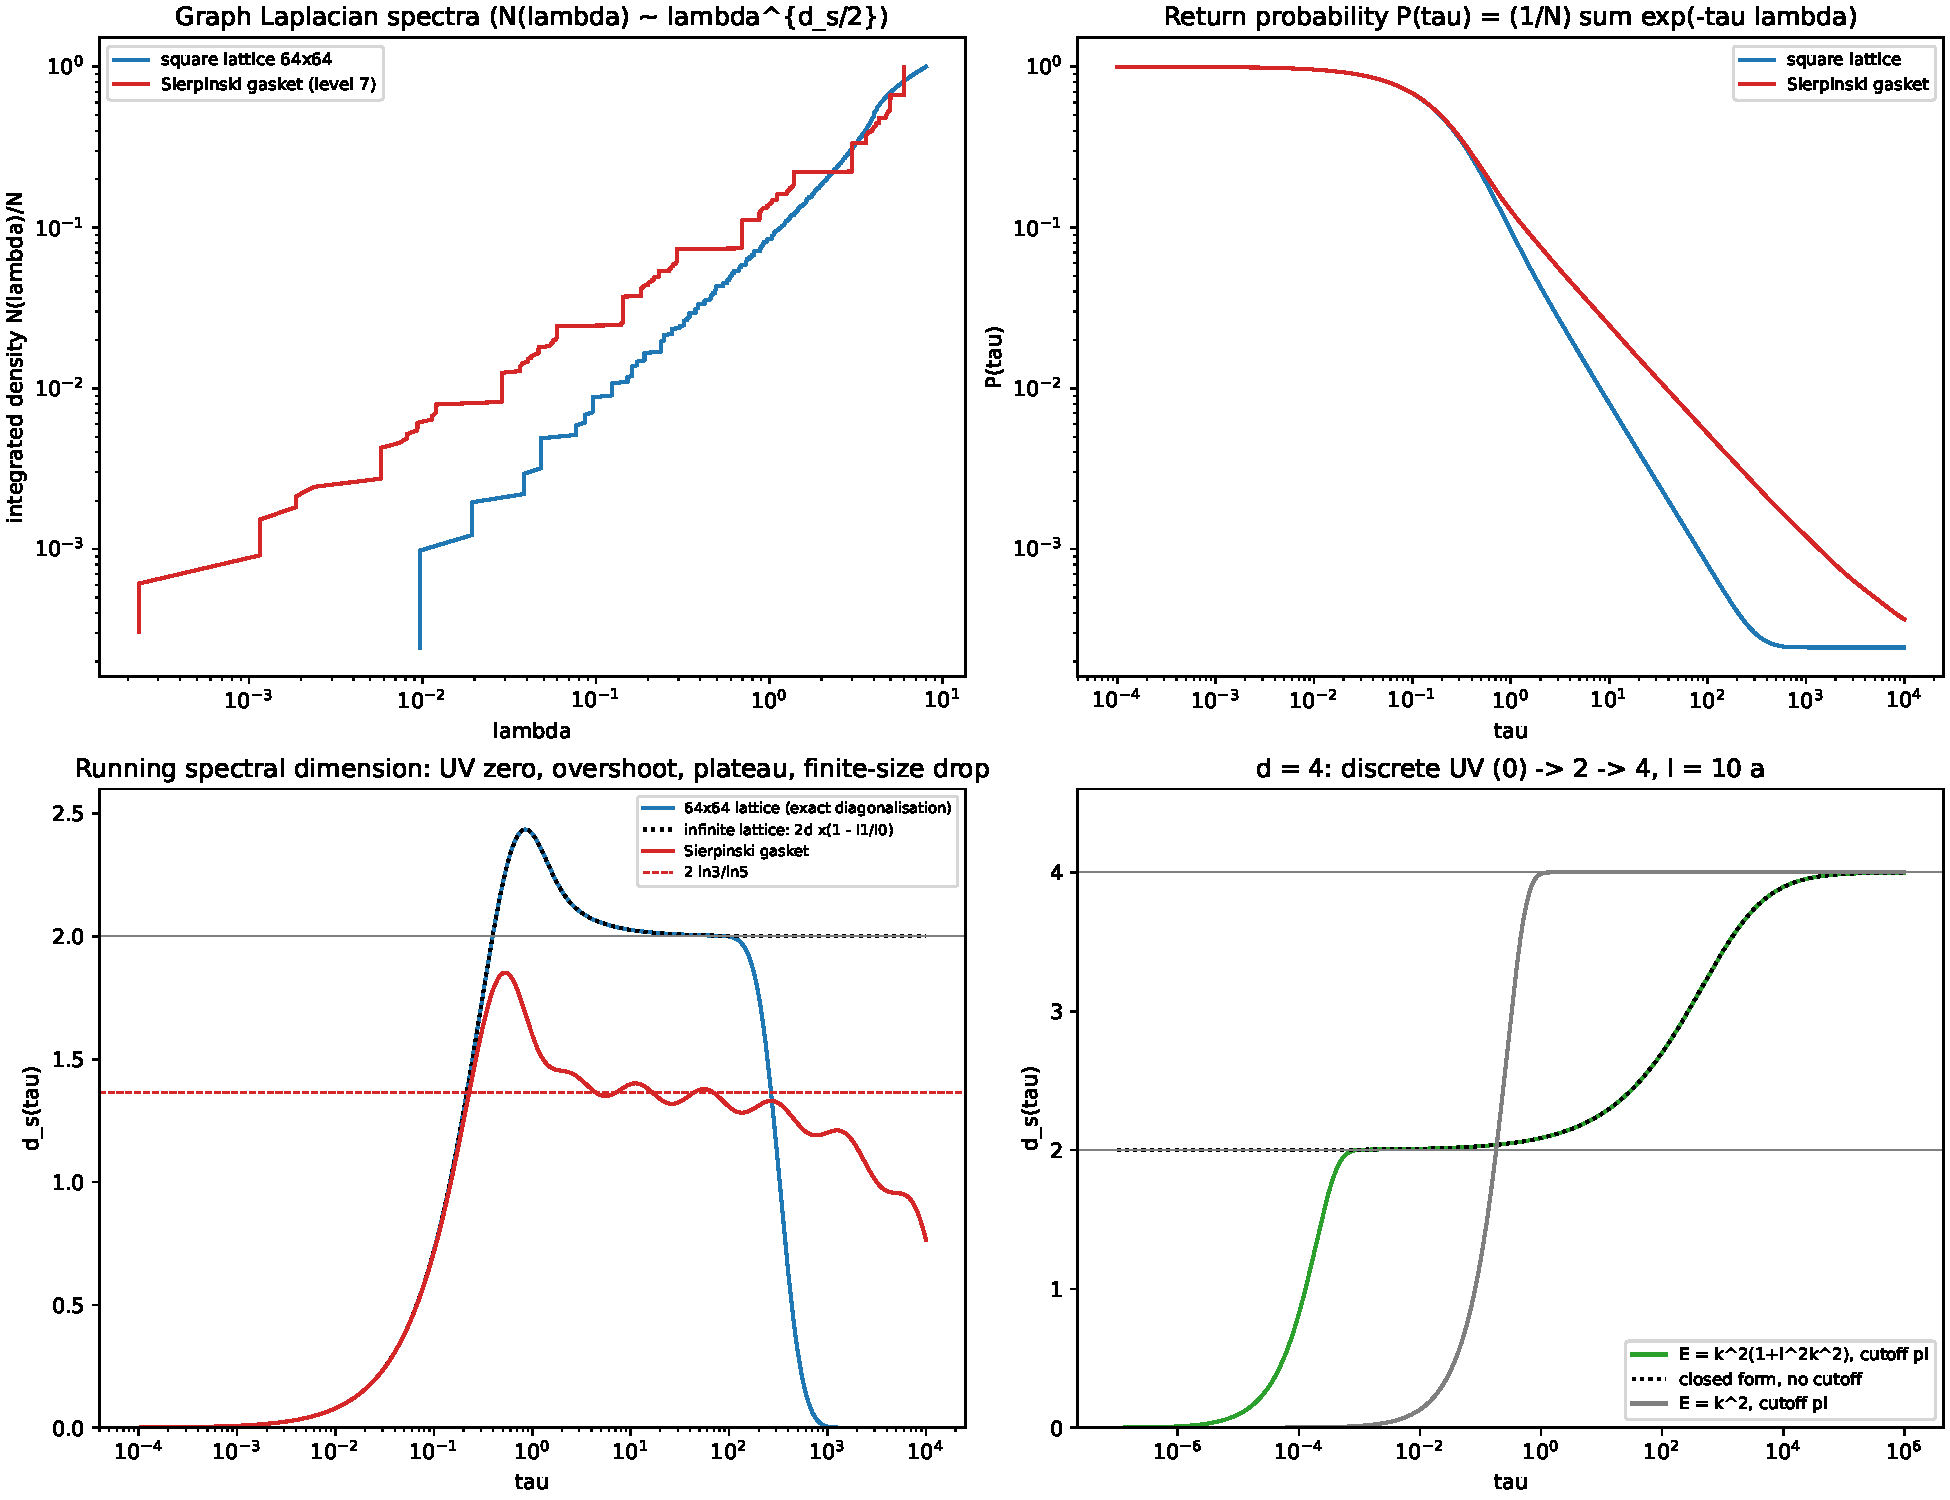
\includegraphics[width=\textwidth]{quantum_geometry_crossover}
\caption{Top left: integrated spectral densities of the $64\times64$ periodic lattice and the level-7 Sierpinski
gasket. Top right: return probabilities. Bottom left: running spectral dimension. The lattice (exact
diagonalisation) coincides with the infinite-lattice formula~\eqref{eq:lattice} until finite-size effects set
in near $\tau\sim10^2$; note the overshoot above $d=2$. The gasket oscillates around $2\ln3/\ln5$. Bottom right:
$d=4$ with $E=k^2(1+\ell^2k^2)$, $\ell=10a$, and cutoff $|k|\le\pi/a$ (green), the closed form~\eqref{eq:erfc}
(dotted), and $E=k^2$ with the same cutoff (grey).}
\label{fig:main}
\end{figure}
\begin{figure}[t]
\centering
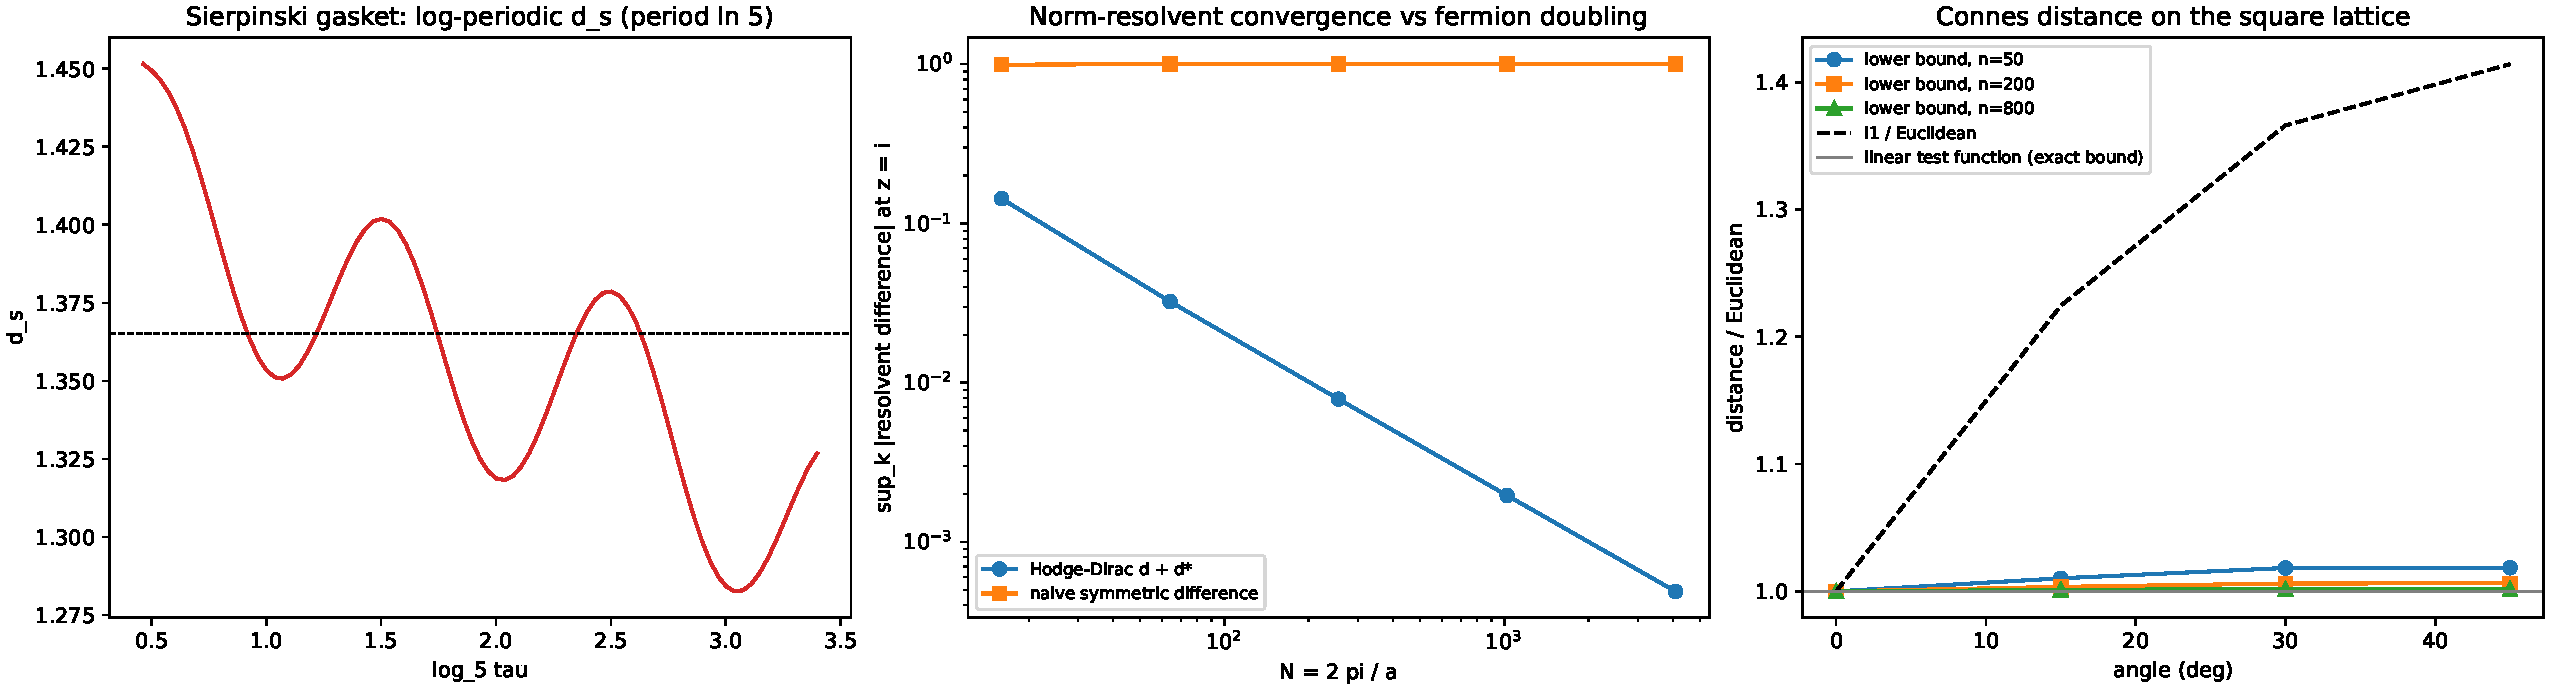
\includegraphics[width=\textwidth]{dirac_and_connes}
\caption{Left: log-periodic oscillation of $d_s$ on the Sierpinski gasket (period $\ln5$). Middle: norm-resolvent
error at $z=i$ on the circle for the lattice Hodge--Dirac operator (convergent, $O(a)$) and the naive
symmetric-difference operator (non-convergent, fermion doubling). Right: lower bound on the Connes distance
on the square lattice relative to the Euclidean distance, compared with the $\ell^1$ distance.}
\label{fig:dirac}
\end{figure}

\section{Discussion and limitations}
\label{sec:discussion}
\begin{enumerate}
\item The identity $d_s=2\tau\langle\lambda\rangle_\tau$ shows that the spectral dimension is a property of the spectral density
alone. It is insensitive to eigenvectors, and hence to geometric information beyond the spectrum. Two
geometries with the same spectrum have the same running $d_s$.
\item The ultraviolet zero and the infrared drop in Corollary~\ref{cor:limits} are generic artefacts. Reported
ultraviolet values of $d_s$ should be read from plateaus well above the cutoff scale and below the finite-size
scale.
\item Theorem~\ref{thm:resolvent} concerns flat tori. Extending norm-resolvent convergence to curved manifolds
and random triangulations, as in CDT, and controlling fermion doubling there, are open problems.
\item The conjectured Euclidean limit of the Connes distance on $\ZZ^d$ is supported by lower bounds only.
\item The functional~\eqref{eq:Gamma} is a truncation, not a derivation from the CDT transition.
\item \emph{Connections within the series.} Log-periodic oscillations of $d_s$ on self-similar graphs are the
heat-kernel counterpart of the complex dimensions of~\cite{Chen2026_holo}. The equipartition form of $d_s$ is an
instance of the thermodynamic formalism used for entanglement spectra in~\cite{Chen2026_multi}. Whether a
computable graph can have an uncomputable spectral dimension, in analogy with the uncomputable fractal
dimensions of~\cite{Chen2026_chaitin}, is left open.
\end{enumerate}

\section*{Data and code availability}
All numbers and figures are produced by the Python script \texttt{quantum\_geometry\_crossover.py}, available
at \url{https://github.com/Ruqing1963/quantum-geometry-crossover} and archived on Zenodo under DOI
\href{https://doi.org/10.5281/zenodo.23195881}{10.5281/zenodo.23195881}.

\appendix
\section{Numerical methods}
\begin{itemize}
\item \emph{Graphs.} The periodic $64\times64$ square lattice and the level-7 Sierpinski gasket (built recursively
on integer coordinates; $N=(3^{8}+3)/2=3282$) are diagonalised exactly with LAPACK (\texttt{numpy.linalg.eigvalsh}).
The lattice eigenvalues agree with the analytic spectrum to $10^{-13}$.
\item \emph{Heat kernel.} $P(\tau)=\frac1N\sum_ke^{-\tau\lambda_k}$ on 321 logarithmically spaced points in $[10^{-4},10^4]$.
$d_s$ is computed both by centred differences in $\ln\tau$ and from~\eqref{eq:equi}; the two agree to $1.5\times10^{-3}$.
\item \emph{Modified dispersion.} Radial integrals with cutoff $\pi/a$ are evaluated by adaptive quadrature
(relative tolerance $10^{-11}$, no absolute tolerance), split at $k=\tau^{-1/2}$, on $\tau\in[10^{-7},10^6]$. Tails with
$\tau E>700$ are omitted, since they underflow.
\item \emph{Dirac operators.} Resolvent differences are evaluated mode by mode on the circle, including the bound
$1/|k|$ for continuum modes outside the Brillouin zone.
\item \emph{Connes distance.} The upwind recursion is checked to satisfy the admissibility constraint at every
vertex; values are reported at the lattice point on each ray at the edge of the grid.
\end{itemize}

\begin{thebibliography}{99}
\bibitem{AJL} J.~Ambj{\o}rn, J.~Jurkiewicz, R.~Loll, ``Spectral dimension of the universe'', Phys.\ Rev.\ Lett.\ 95 (2005) 171301, arXiv:hep-th/0505113.
\bibitem{LauscherReuter} O.~Lauscher, M.~Reuter, ``Fractal spacetime structure in asymptotically safe gravity'', JHEP 10 (2005) 050, arXiv:hep-th/0508202.
\bibitem{Horava} P.~Ho\v{r}ava, ``Spectral dimension of the universe in quantum gravity at a Lifshitz point'', Phys.\ Rev.\ Lett.\ 102 (2009) 161301, arXiv:0902.3657.
\bibitem{Modesto} L.~Modesto, ``Fractal structure of loop quantum gravity'', Class.\ Quant.\ Grav.\ 26 (2009) 242002, arXiv:0812.2214.
\bibitem{Benedetti} D.~Benedetti, ``Fractal properties of quantum spacetime'', Phys.\ Rev.\ Lett.\ 102 (2009) 111303, arXiv:0811.1396.
\bibitem{Calcagni} G.~Calcagni, ``Fractal universe and quantum gravity'', Phys.\ Rev.\ Lett.\ 104 (2010) 251301, arXiv:0912.3142.
\bibitem{Carlip} S.~Carlip, ``Dimension and dimensional reduction in quantum gravity'', Class.\ Quant.\ Grav.\ 34 (2017) 193001, arXiv:1705.05417.
\bibitem{CES} G.~Calcagni, A.~Eichhorn, F.~Saueressig, ``Probing the quantum nature of spacetime by diffusion'', Phys.\ Rev.\ D 87 (2013) 124028, arXiv:1304.7247.
\bibitem{ConnesBook} A.~Connes, \emph{Noncommutative Geometry}, Academic Press, San Diego (1994).
\bibitem{Connes96} A.~Connes, ``Gravity coupled with matter and the foundation of non-commutative geometry'', Commun.\ Math.\ Phys.\ 182 (1996) 155, arXiv:hep-th/9603053.
\bibitem{AlexanderOrbach} S.~Alexander, R.~Orbach, ``Density of states on fractals: fractons'', J.\ Physique Lett.\ 43 (1982) 625, doi:10.1051/jphyslet:019820043017062500.
\bibitem{RammalToulouse} R.~Rammal, G.~Toulouse, ``Random walks on fractal structures and percolation clusters'', J.\ Physique Lett.\ 44 (1983) 13, doi:10.1051/jphyslet:0198300440101300.
\bibitem{ADT} E.~Akkermans, G.~V.~Dunne, A.~Teplyaev, ``Physical consequences of complex dimensions of fractals'', EPL 88 (2009) 40007, arXiv:0903.3681.
\bibitem{NielsenNinomiya} H.~B.~Nielsen, M.~Ninomiya, ``Absence of neutrinos on a lattice (I). Proof by homotopy theory'', Nucl.\ Phys.\ B 185 (1981) 20.
\bibitem{Stelle} K.~S.~Stelle, ``Renormalization of higher derivative quantum gravity'', Phys.\ Rev.\ D 16 (1977) 953.
\bibitem{AJJL} J.~Ambj{\o}rn, S.~Jordan, J.~Jurkiewicz, R.~Loll, ``A second-order phase transition in CDT'', Phys.\ Rev.\ Lett.\ 107 (2011) 211303, arXiv:1108.3932.
\bibitem{DLMF} NIST Digital Library of Mathematical Functions, \S10.40, \url{https://dlmf.nist.gov/10.40}.
\bibitem{GR} I.~S.~Gradshteyn, I.~M.~Ryzhik, \emph{Table of Integrals, Series, and Products}, 7th ed., Academic Press (2007), formula 3.462.1.
\bibitem{Chen2026_holo} R.~Chen, ``Holographic entanglement of fractal regions: Complex dimensions, non-local counterterms and cosmic-brane multifractality'' (2026), doi:10.5281/zenodo.23189575.
\bibitem{Chen2026_multi} R.~Chen, ``Multifractal large deviations in quantum entanglement: Ideal Fermi-gas mapping, Markov tensor cascades, and quartic Casimir symmetry'' (2026), doi:10.5281/zenodo.23193512.
\bibitem{Chen2026_chaitin} R.~Chen, ``Uncomputable fractal dimensions, Kolmogorov complexity cascades, and the Chaitin barrier in physical systems'' (2026), doi:10.5281/zenodo.23194419.
\end{thebibliography}
\end{document}
